%\documentclass[a4paper,12pt]{report}
\documentclass[finnish,12pt]{article}
%\usepackage[utf8]{inputenc}
\usepackage[latin1]{inputenc}
\usepackage[finnish]{babel}
\usepackage{ae,aecompl}

\usepackage[pdftex]{graphicx}
\usepackage{url}
%% Matematiikan fontteja, symboleja ja muotoiluja lis��, n�it� tarvitaan usein
\usepackage{amsfonts,amssymb,amsbsy}
%% Taulukon paketti
%\usepackage{multirow}

%% Vaakasuunnan mitat, �L� KOSKE!
\setlength{\hoffset}{-1in}
\setlength{\oddsidemargin}{35mm}
\setlength{\evensidemargin}{20mm}
\setlength{\textwidth}{15cm}
%% Pystysuunnan mitat, �L� KOSKE!
\setlength{\voffset}{-1.5in}
%\setlength{\headsep}{7mm}
%\setlength{\headheight}{1em}
\setlength{\topmargin}{25mm}
\setlength{\textheight}{24cm}
%% Vasensuora-asettelu, joka opinn�ytteess� vaaditaan. �L� KOSKE
\setlength{\parindent}{0pt}
\setlength{\parskip}{1ex}

%% bibtex-tyyli
\bibliographystyle{apalike}

% Title Page
\title{S-113.2210 Seminaarity�: arpikudos aivoelektrodeissa}
\author{Mikko Tuohimaa}
\date{7.4.2011}


\begin{document}
\maketitle
\pagenumbering{roman}
%\setcounter{page}{1}
\begin{abstract}
Aivoihin implantoitavien elektrodien ymp�rille syntyv� arpikudos on yksi suurimmista syist� pitk�aikaisten implanttien suorituskyvyn huonontumiseen, syyn� sen erist�v� vaikutus. T�ss� ty�ss� k�yd��n l�pi nykyiset implanttityypit, arpikudoksen muodostumisprosessi ja kartoitetaan eri menetelmi� sen ehk�isemiseksi.
\end{abstract}

\clearpage
\tableofcontents
\clearpage

% Aloitetaan arabialainen numerointi vasta t�st�
\pagenumbering{arabic}
\setcounter{page}{1}

% Osiot ovat omina tiedostoinaan, jolloin niit� voi muokata samanaikaisesti
% ja my�s j�rjestell� helposti
\section{Johdanto}

Aivoihin implantoidut pii-, polymeeri- ja mikrolankaelektrodit ovat paras ja p��asiallinen tapa ker�t� tarkkaan lokalisoitua tietoa aivojen s�hk�isest� aktiivisuudesta. T�t� tietoa pystyt��n puolestaan k�ytt�m��n hyv�ksi paitsi kliinisess� tutkimuksessa, my�s esim. ohjattavien proteesien k�ytt�liittym�n�. Eritoten j�lkimm�isess� tarkoituksessa implantointi on tarkoitettu pysyv�ksi, joten elektrodien pitk�n ajan toiminnallisuus on t�rke��.

Suurimpana haasteena kroonisesti implantoitujen elektrodien toiminnassa on elimist�n immuunivaste ja varsinkin keskushermoston uniikki vierasesinereaktio. Tutkimuksissa on havaittu, ett� elektrodista saatava signaali yleens� heikkenee ajan kuluessa niin, ett� jo 4 viikon j�lkeen elektrodi saattaa olla k�ytt�\-kel\-vo\-ton. T�m� suurimmalta osin johtuu siit�, ett� elektrodin ymp�rille muodostuu arpikudosta, joka lis�� elektrodin ja neuronien v�list� et�isyytt� ja toimii my�s s�hk�isen� eristeen� - jo 50 $\mu$m:n suuruusluokkaa oleva arpikudoskerros voi heikent�� signaalia merkitt�v�sti. T�m� ty� esittelee eri elektrodityyppej� ja tapoja, joilla arpikudoksen muodostumista voidaan v�hent��. \cite{Polikov}

\section{Implanttityypit}

Perinteisesti v�liaikaisia mittauksia on tehty yksitt�isell� mikrolangalla tai lasisella mikropipettielektrodilla. On kuitenkin selv��, ett� implantoidessa elektrodit pysyv�sti halutaan samassa operaatiossa istuttaa mahdollisimman paljon dataa tarjoava anturijoukko: p��paino onkin k��ntynyt monielektrodisiin sovelluksiin, jotka voidaan toteuttaa mikrolanka- tai piipohjaisilla tekniikoilla. T�ll�in elektrodijoukossa voikin olla jopa sata mittauspistett� hyvin l�hell� toisiaan, mill� saadaan sek� kasvatettua signaalin voimakkuutta ett� tutkittua neuroniverkkojen toimintaa. \cite{Nicolelis}

Yhteist� kaikille implanttityypeille on se, ett� itse elektrodi on pieni alue tukivarren p��ss� muun implantin ollessa s�hk�isesti eristetty. T�m� mahdollistaa paikallisen mittaamisen ja parempilaatuisen signaalin.

\subsection{Mikrolangat}

Mikrolangat ovat joidenkin mikrometrien paksuisia metallilankoja (yleisimpin� materiaaleina platina, kulta, volframi, iridium ja ruostumaton ter�s), jotka on p��llystetty eristeell�, yleens� lasilla (kuva \ref{fig:microwire}). Mikrolangoista voidaan tehd� pitki�, mik� mahdollistaa mittaukset syvemm�lt� aivoista, mutta koska ne ovat joustavia ja aivokudos on heterogeenist�, ei niiden tarkka implantointi ole mahdollista.

\begin{figure}[htcb]
 \begin{center}
  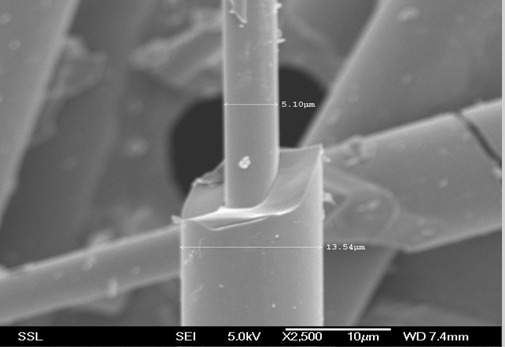
\includegraphics[scale=0.75]{microwire.jpg}
  \caption{Elektronimikroskooppikuva lasip��llysteisest� mikrolankaelektrodista. L�hde: http://www.jyi.org/research/re.php?id=1493}
  \label{fig:microwire}
 \end{center}
\end{figure}


\subsection{Piipohjaiset implantit}

Piipohjaiset implantit valmistetaan elektroniikasta ja MEMS-teknologiasta tutuilla menetelmill�. Kyseisill� tekniikoilla saadaan aikaan tarkkoja, eritt�in pieni� rakenteita, joiden s�hk�iset ominaisuudet ovat hyvin hallittavissa. Kuvassa \ref{fig:silicon_probe} n�kyy perinteisen muotoinen piipiikkielektrodi, johon on my�s lis�tty kemiallinen sensori.

\begin{figure}[htcb]
 \begin{center}
  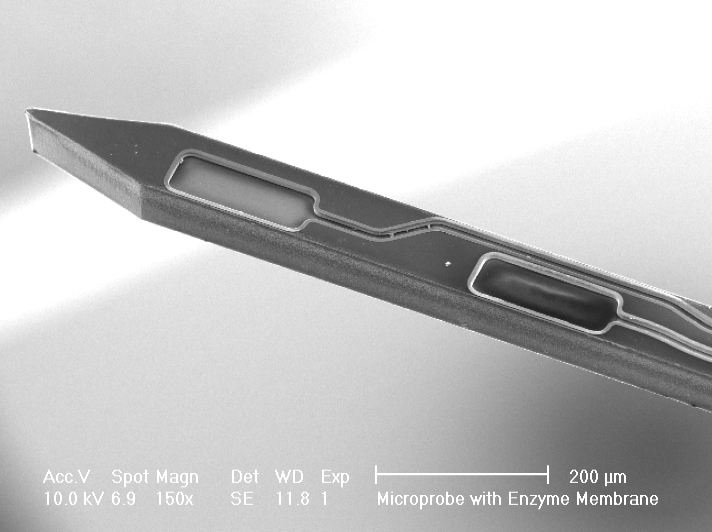
\includegraphics[scale=0.5]{silicon_probe.jpg}
  \caption{Elektronimikroskooppikuva piipohjaisesta elektrodista, joka sis�lt�� my�s kemiallisen sensorin. L�hde: http://samlab.epfl.ch/page-15473-en.html}
  \label{fig:silicon_probe}
 \end{center}
\end{figure}

Pii-implantit valmistetaan usein siten, ett� yhdess� elementiss� on monta yksitt�ist� elektrodia oman tukivartensa p��ss� joko jono- tai matriisimuodostelmassa (kuva \ref{fig:silicon_array}). Nykyisill� menetelmill� kunkin piikin korkeus on yksil�llisesti valittavissa ja yhdess� piikiss� voi olla useita mittauspisteit�, joten neuroverkkojen 3D-mittaukset ovat mahdollisia.

Piipohjaisia valmistusmenetelmi� k�ytett�ess� voi itse implantin materiaalina olla my�s jokin muu kuin pii, kuten polymeeri tai metalli. Valmistusmenetelm�t kuitenkin rajoittavat materiaalivalikoimaa jonkin verran.

\begin{figure}[htcb]
 \begin{center}
  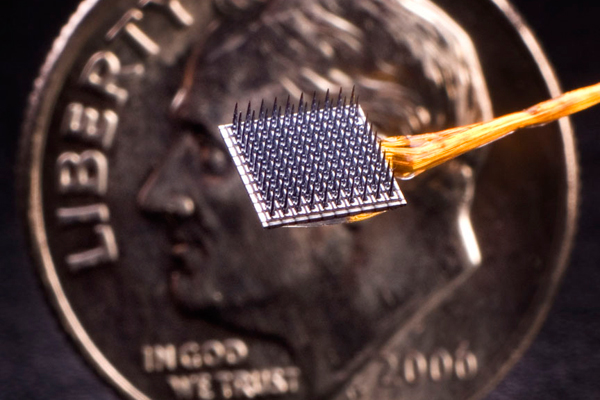
\includegraphics[scale=0.5]{silicon_array.jpg}
  \caption{Piielektrodimatriisi. L�hde: http://www.newscientist.com/blogs/ shortsharpscience/2011/03/power-of-thought-neural-implan.html}
  \label{fig:silicon_array}
 \end{center}
\end{figure}

\subsection{Polymeeri-implantit}

Polymeereja on tutkittu implanttimateriaaleina jonkin verran. Niiden ehdottomana etuna on elastisuuden tuoma parempi kimmoyhteensopivuus kudoksen kanssa, mutta heikkoutena implantoinnin vaikeus: joustavaa implanttia ei voi ty�nt�� suoraan aivokalvon l�pi, vaan v�yl� t�ytyy puhkaista erikseen. T�m� on sek� haastavampaa ett� aiheuttaa enemm�n tuhoa kudoksessa kuin pii- ja mikrolankaimplanttien tapauksessa. \cite{Polikov}

%\clearpage
\section{Implantointi ja keskushermoston immuunivaste}

Implantoinnin ja elektrodien itsens� aiheuttama immuunivaste aivoissa on suurin elektrodin toimintaa haittaava tekij�. Siisp� elektrodien suorituskyvyn maksimoimiseksi on t�rke�� ymm�rt�� ne biologiset mekanismit, jotka ajavat immuuniprosessia.

On huomattava, ett� neuronit muodostavat vain alle 25\% aivokudoksesta; loput ovat verenkiertoon liittyvi� soluja sek� gliosyyttej�, hermotukisoluja, jotka ovat aivojen immuunivasteen merkitt�vimm�t osallistujat. N�ist� astrosyytit muodostavat matriksia (arpikudosta) vauriokohtaan ja mikrogliasolut toimivat sytotoksisina soluina tai fagosyyttein� tuhoten vaurioitunutta kudosta.

Implantointiprosessi on usein v�kivaltainen - neulamaiset elektrodit ty�nnet��n aivokudoksen l�pi kohteeseensa, mik� rikkoo hiussuonia,  aivojen tukikudosta ja solurakenteita. Lis�ksi implantti syrj�ytt�� tielt��n kudosta aiheuttaen painetta implantin v�litt�m�ss� l�heisyydess� olevassa kudoksessa. T�m� mekaaninen vaurio aiheuttaa keskushermostolle ominaisen vasteen, joka muistuttaa paljon muiden kudosten paranemisprosessia. Mainittakoon, ett� vauriokohtaan kertyy nestett� aiheuttaen turvotusta, mik� edelleen pahentaa kudokseen kohdistuvaa painetta.\cite{Polikov}

Paranemisprosessi on tehokas, ja implantointireitin vauriot yleens� korjautuvat joidenkin viikkojen aikana. Varsinaisena ongelmana onkin, ett� implantti jota mikrogliasolut eiv�t saa tuhottua saa aikaan kroonisen vierasesinevasteen, jossa mikrogliasolut eritt�v�t jatkuvasti proteolyyttisi� entsyymej� tuhoten samalla ymp�r�iv�� hermokudosta \cite{McConnell} ja astrosyytit muodostavat implantin ymp�rille arpikudosta. T�m� reaktio tulee esille vasta varsinaisen immuunireaktion j�lkeen ja on suurin syyllinen ep�onnistuneisiin implantointeihin. Kuvaavaa on, ett� er��ss� tutkimuksessa 25\%:ssa implantoiduista piielektrodeista oli merkkej� aktivoituneista mikrogliasoluista viel� 6 kuukautta implantoinnin j�lkeen. \cite{Schmidt} Yleisesti ottaen jo kuudessa viikossa arpikudos saattaa olla niin paksu, ett� se haittaa pysyv�sti elektrodin toimintaa. \cite{Turner}

\subsection{Implantointimenetelm�n vaikutus}

Tutkimukset osoittavat, ett� veren seerumilla on merkitt�v� osuus arpeutumisen edist�misess� ja veri my�s aiheuttaa tulehdusreaktion kudoksessa. T�m�n takia mit� v�hemm�n verisuonia katkeaa implantoinnin yhteydess�, sit� pienempi on immuunireaktio ja sit� v�hemm�n arpikudosta syntyy. Implantointimenetelm� saattaa vaikuttaa syntyneeseen vaurioon ja siten implantoinnin onnistumiseen, mutta vertailukelpoisia tuloksia ei juuri ole. Eri tutkimusryhm�t ovat kokeilleet eri implantointinopeuksia n. 100 $\mu$m/s ja 8,3 m/s v�lill�, mutta koska tarkasteltava systeemi on niin monimutkainen, on kullakin menetelm�ll� ja nopeudella etunsa ja haittansa. \cite{Polikov}

%Bioaktiiviset pinnat houkuttelevat neuroneita l�helleen ja siten maksimoivat signaalin lyhyell� aikav�lill�, mutta eiv�t hidasta arpikudoksen muodostumista.

%Ongelma: bioaktiivisten aineiden saaminen elektrodille jatkuvalla sy�t�ll�. Mikrofluidistiikka?
\section{Implantin mekaniikka}

Elektroniikassa ja MEMS-teknologiassa yleisesti k�yt�ss� olevat piin muokkausmenetelm�t ovat avanneet uusia mahdollisuuksia piipohjaisten implanttien rakenteelle. Kokeiluja on tehty niin elektrodivarren poikkileikkauksen kuin 3D-muodon suhteen, mutta yhteisten standardien puuttuessa tulokset eiv�t ole kesken��n kovinkaan vertailukelpoisia. %\cite{Polikov}

Implantin rakenteessa olennaista on sen mekaaniset ominaisuudet ja dimensiot. Reunaehtona on, ett� implantin pit�� olla k�ytt�tarkoitukseensa tarpeeksi vankkaa tekoa, mutta muuten yleinen k�sitys on, ett� mit� pienempi implantti on, sit� paremmin se soveltuu pitk�aikaiseen k�ytt��n. My�s erilaiset materiaalivalinnat vaikuttavat sen ominaisuuksiin, erityisesti kimmomoduuliin, mill� on my�s oma vaikutuksensa bioyhteensopivuuteen. \cite{Polikov} \cite{Seymour}

\subsection{Mikroliike}

Aivot eiv�t ole staattisessa tilassa, vaan liikkuvat sek� paikallisesti ett� kokonaisuutena suhteessa kalloon syd�menly�ntien, hengityksen ja potilaan liikkeiden vaikutuksesta aiheuttaen paikallista painetta ja voimia. Implantoitavat elektrodit ovat yleens� k�yt�nn�n syist� hyvin paljon aivokudosta j�ykempi�, mink� johdosta ymp�r�iv�t voimat saavat aikaan implantin mikroliikett� suhteessa kudokseen. T�m� puolestaan rikkoo soluv�liaineen rakenteita implantin v�litt�m�ss� l�heisyydess� ja aiheuttaa immuunireaktion. Materiaalivalinnalla voidaan vaikuttaa implantin j�ykkyyteen ja joitakin kokeiluja onkin tehty mm. polymeereilla, mutta toistaiseksi pii on yleisin materiaali sen ty�st�ominaisuuksien vuoksi.

\subsection{Implantin johdotus}

Yksi mikroliikett� aikaansaava tekij� on implantin johdotus kallosta ulos. Implantin mittaustulokset pit�� saada hy�tyk�ytt��n, eik� langattomuus ole t�ss� mittakaavassa vaihtoehto - siisp� johdotus on vedett�v� kallon l�pi, ja kun elektrodi on mekaanisesti kiinni kallossa ja aivot liikkuvat suhteessa kalloon, on yht�l� vaikea ratkaistavaksi. Erilaisia joustavia, esim. polymeeripohjaisia johdotuksia on ehdotettu \cite{Lee}, mutta mit��n hyv�� ratkaisua t�h�n ongelmaan ei viel� ole.

Yhten� vaihtoehtona voisi olla elektrodien ohjauselektroniikan sijoittaminen aivojen pinnalle, energian tarjoaminen induktiivisesti ja datan siirto radioteitse. T�ll�in kallon ja elektrodin v�lill� ei olisi suoraa mekaanista yhteytt�, mutta toisaalta implantoitavan materiaalin m��r� kasvaisi huomattavasti, mik� puolestaan lis�isi sek� implantoinnin haasteellisuutta ett� mahdollisesti kokonaisvierasesinevastetta.

\subsection{Ristikkorakenne}

Seymour ja Kipke kokeilivat tutkimuksessaan \cite{Seymour} elektrodirakennetta, jossa perinteisin piimenetelmin valmistetun paryleenivarren yhdess� reunassa on hyvin kapeaelementtinen ristikkorakenne (kuva \ref{fig:ristikko}). Hypoteesina oli, ett� mit� pienempi elektrodipinnan dimensio on, sit� vaikeampaa on astrosyyttien tarttua siihen ja sit� kautta muodostaa arpikudoskoteloa sen ymp�rille. Implantti ei voi kuitenkaan kokonaisuudessaan olla kovinkaan ohut, koska implantointi vaatii tietyt mekaaniset ominaisuudet. Tutkimuksessa k�ytetty rakenne osoittautui hyv�ksi, koska sill� saavutettiin vain 4 $\mu$m kapea pinta elektrodin kokonaisj�ykkyyden k�rsim�tt� juurikaan.

\begin{figure}[htcb]
 \begin{center}
  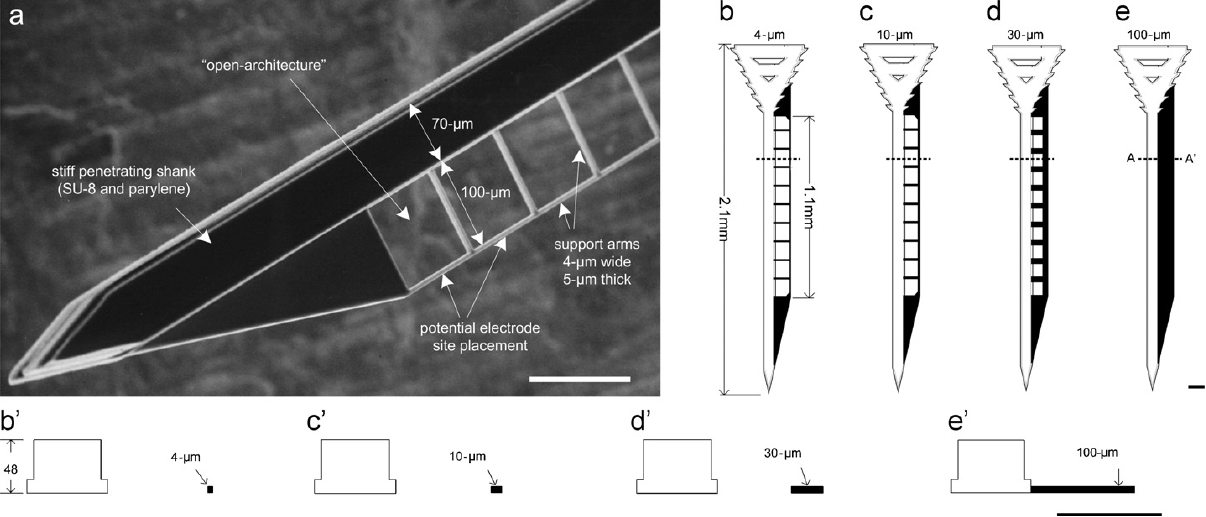
\includegraphics[scale=0.4]{ristikko_rakenne.png}
  \caption{Seymourin ja Kipken k�ytt�m� epoksi-paryleenipohjainen ristikkorakenne. \cite{Seymour}}
  \label{fig:ristikko}
 \end{center}
\end{figure}

Kuvassa \ref{fig:ristikko_vaste} n�kyy, miten Seymourin ja Kipken tutkimuksessa immuunivaste on keskittynyt elektrodin varren ymp�rille itse elektrodin j��dess� huomattavasti vapaammaksi. T�m� tukee alkuper�ist� hypoteesia, mutta on my�s huomattava ett� kapeat tukivarret ovat perinteist� joustavampia, mik� saattaa osaltaan vaikuttaa parantuneeseen vasteeseen. On mahdollista, ett� joustavampi rakenne v�hent�� mikroliikkeen aikaansaamaa vauriota soluv�liaineessa ja siten my�s kroonista tulehdusreaktiota elektrodipinnan v�litt�m�ss� l�heisyydess�.

\begin{figure}[h]
 \begin{center}
  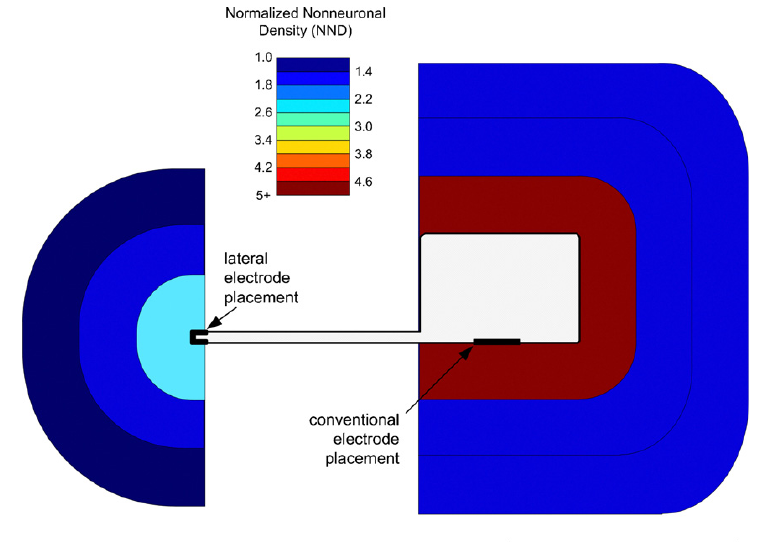
\includegraphics[scale=0.5]{ristikko_tulokset.png}
  \caption{Seymourin ja Kipken tulokset: ei-neuronaalisen kudoksen tiheys varren ja ristikkorakenteen ulkoreunan ymp�rill�.�Tulokset osoittavat rakenteen aiheuttavan v�hemm�n koteloitumista elektrodipinnan l�heisyydess� kuin perinteisen elektrodisijoittelun tapauksessa. \cite{Seymour}}
  \label{fig:ristikko_vaste}
 \end{center}
\end{figure}

Ristikkorakenteen tekemisess� k�ytetyill� valmistusmenetelmill� on mahdollista tehd� my�s muunlaisia palkkirakenteita tasossa, esimerkiksi kolmiopalkkirakenteita. Suorakulmainen ristikkorakenne on kuitenkin siin� mieless� optimaalinen, ett� jos elektrodi sijoitetaan kahden tukipalkin v�lille, rakenne minimoi materiaalin m��r�n elektrodin l�heisyydess�. 3D-rakenteetkin ovat teoriassa mahdollisia, mutta k�yt�nn�ss� niin kalliita valmistaa, ett� niit� ei viel� kannata tutkia kovinkaan paljoa.
\section{Bioaktiiviset pinnoitteet}

Yksi keino lis�t� aivoelektrodien pitk�n ajan suorituskyky� on muokata aivojen reaktiota implanttiin erilaisilla bioaktiivisilla pinnoitteilla. Pinnoitteiden tarkoituksena voi olla lis�t� tai v�hent�� neuronien ja/tai astrosyyttien kasvua ja tarttumista, v�hent�� tulehdusreaktiota, tai edellisten yhdistelm�. Monia yksitt�isi� aktiivisia aineita on tutkittu, muun muassa dekstraania, hyaluronihappoa ja deksametasonia \cite{Grand} sek� erilaisia hydrogeelej�. Lis�ksi implantteja on pinnoitettu teflonilla ja muilla tarttumista est�vill� polymeereilla. \cite{Polikov}

\subsection{Tulehdusl��kkeet}

Tulehdusl��kkeiden tarkoitus on hillit� implantoinnin aikaansaamaa tulehdusreaktiota ja immuunivastetta. Grand ryhmineen tutki mm. deksametasonipinnoitteen vaikutusta neuronien kuolleisuuteen, ja tuloksena oli ett� t�m�n synteettisen kortikosteroidin l�sn�olo v�hensi neuronikatoa implantin v�litt�m�st� l�heisyydest�. T�m� tarkoittaa sit�, ett� lyhyell� aikav�lill� signaalin laatu oli parempi, mutta pidemm�ll� aikav�lill� deksametasonin ei havaittu vaikuttavan arpikudoksen muodostumiseen eik� siten parantavan pidempiaikaista suorituskyky�. \cite{Grand} T�m�n syyn� saattaa olla yksinkertaisesti l��keaineen kuluminen pinnalta pois (ks. kappale \ref{Mikrofluidistiikka}).

\subsection{Kiinnittymist� est�v�t pinnat}

Grandin tutkimusryhm� tutki my�s dekstraanipinnoitetta. Dekstraani on polysakkaridi, jota k�ytet��n yleisesti verenohentajana, ja pinnalle sidottuna se ehk�isee jossain m��rin solujen, mukaanlukien astrosyyttien, kiinnittymist� ja levi�mist� ja saattaa siten vaikuttaa arpikudoksen muodostumiseen.

Lun ryhm� puolestaan kehitti poly(vinyl alcohol)/poly(acrylic acid) -hydrogeelin, joka ehk�isi tehokkaasti proteiinien adsorptiota (jopa 85\%) ja sit� kautta todennetusti v�hensi jonkin verran arpikudoksen muodostumista. \cite{Lu}

\subsection{Bioyhteensopivuutta lis��v�t pinnat}

Joitakin soluv�liainetta simuloivia pintoja on kokeiltu aivoelektrodeissa. Hyaluronihappoa esiintyy runsaasti aivojen soluv�liaineessa ja se my�s osallistuu paranemisprosessiin. On osoitettu, ett� sen injektoiminen vaurioituneelle alueelle v�hent�� arpikudoksen muodostumista, mutta Grandin kokeessa sill� pinnoitetun elektrodin ymp�rille syntyi vain marginaalisesti v�hemm�n arpikudosta kuin pinnoitetun referenssielektrodin ymp�rille. \cite{Grand}

Jotkin pinnoitteet my�s lis��v�t neuronitiheytt� implantin l�heisyydess� ja siten kasvattavat mitatun signaalin voimakkuutta, mutta n�m�kin toimivat vain lyhyell� aikaj�nteell�. \cite{Polikov}

\subsection{Mikrofluidistiikka ja nanopartikkelit}
\label{Mikrofluidistiikka}
Monissa pinnoitteissa pidemm�n ajan ongelmana on, ett� ne kuluvat ajan my�t� pois ja siten niiden vaikutus lakkaa. Pysyv�n implantin suorituskyky ei saisi kuitenkaan heiket� merkitt�v�sti ajan my�t�, joten pinnoitteiden vaikutusaikaa olisi syyt� kasvattaa. Nanopartikkelit ja mikrofluidistiikka ovat mahdollisia ratkaisuja t�h�n ongelmaan.

Nanopartikkelit ovat t�ss� yhteydess� nanokoon hiukkasia, joiden sis�lle vaikuttava aine on pakattu. Partikkelit puolestaan on vangittu matriksiin, joka hajoaa elimist�ss� hitaalla vakionopeudella vapauttaen partikkeleita tasaiseen tahtiin. N�in itse vaikuttavan aineen annostelua pystyt��n kontrolloimaan ja vaikutusaikaa pident�m��n, vaikkakaan ei loputtomiin. Esimerkiksi A. Mercanzini ryhmineen on onnistunut tekem��n pinnoitteen, jonka ominaisuudet vaikuttavat lupaavilta t�ss� suhteessa. \cite{Mercanzini}

Mikrofluidistiikka puolestaan tarkoittaa yleens� piipohjaista nesteenk�sittely�. Mikrokoon kanavissa hallitseviksi ilmi�iksi nousevat pintaj�nnitys ja diffuusio painovoiman ja massan hitauden sijaan, mik� tuo uusia ulottuvuuksia nesteen k�sittelyyn. Esimerkiksi mustesuihkutulostimet ovat hyv� esimerkki mikrofluidistiikan arkisovelluksista.

Valmistusteknologian kehittymisen my�t� nyky��n on t�ysin mahdollista lis�t� piipohjaiseen elektrodiin kanava, jota pitkin l��keainetta voidaan annostella mikropumpulla hallitusti suoraan mittauspaikan l�heisyyteen. Mm. Wadhwan ryhm� teki hieman t�m�n suuntaisen kokeen, tosin erillisell� annostelijalla, ja tulokset olivat positiivisia. \cite{Wadhwa}
%\section{Tulevaisuuden n�kymi�}

Jaa-a, saas n�h� mit� tapahtuu.
\section{Johtop��t�kset}

Arpikudoksen syntyminen on merkitt�v� ongelma kroonisesti implantoitujen aivoelektrodien yhteydess�, mutta viime vuosina on kehitelty useita menetelmi� useilla eri l�hestymistavoilla arpeutumisen v�hent�miseksi. Lupaavia tuloksia on saatu sek� uudenmallisten elektrodien, elektrodimateriaalien ett� erilaisten elektrodipinnoitteiden tiimoilta. Todenn�k�isesti paras tulos syntyy yhdistelem�ll� n�it� tekniikoita hallitusti ja kenties tulevaisuudessa ottamalla mikrofluidistiikka avuksi l��keaineiden kohdennetussa annostelussa. My�s implantin johdotukseen tulee kiinnitt�� huomiota, tavoitteena minimoida implantin mikroliike aivokudokseen n�hden.

Yleisesti ottaen ala kehittyy nopeasti luotettavan aivo-tietokone-k�ytt�liittym�n tarjoamien ��rett�mien mahdollisuuksien, kuten ajatuksella ohjattavien keinoraajojen ansiosta ja mit� suurimmalla varmuudella jatkaa kehityst��n tulevina vuosina. Yhten� yksitt�isen� kehityskohteena tieteellisell� yhteis�ll� voisi olla yhdenmukaisten testiolosuhteiden luominen, jotta eri tutkimuksia voitaisiin luotettavasti vertailla.

\clearpage

% liitet��n bibtex-viitteet
\bibliography{biomat_semma}

\end{document}          
